% Template for PLoS
% Version 3.0 December 2014
%
% To compile to pdf, run:
% latex plos.template
% bibtex plos.template
% latex plos.template
% latex plos.template
% dvipdf plos.template
%
% % % % % % % % % % % % % % % % % % % % % %
%
% -- IMPORTANT NOTE
%
% This template contains comments intended 
% to minimize problems and delays during our production 
% process. Please follow the template instructions
% whenever possible.
%
% % % % % % % % % % % % % % % % % % % % % % % 
%
% Once your paper is accepted for publication, 
% PLEASE REMOVE ALL TRACKED CHANGES in this file and leave only
% the final text of your manuscript.
%
% There are no restrictions on package use within the LaTeX files except that 
% no packages listed in the template may be deleted.
%
% Please do not include colors or graphics in the text.
%
% Please do not create a heading level below \subsection. For 3rd level headings, use \paragraph{}.
%
% % % % % % % % % % % % % % % % % % % % % % %
%
% -- FIGURES AND TABLES
%
% Please include tables/figure captions directly after the paragraph where they are first cited in the text.
%
% DO NOT INCLUDE GRAPHICS IN YOUR MANUSCRIPT
% - Figures should be uploaded separately from your manuscript file. 
% - Figures generated using LaTeX should be extracted and removed from the PDF before submission. 
% - Figures containing multiple panels/subfigures must be combined into one image file before submission.
% See http://www.plosone.org/static/figureGuidelines for PLOS figure guidelines.
%
% Tables should be cell-based and may not contain:
% - tabs/spacing/line breaks within cells to alter layout or alignment
% - vertically-merged cells (no tabular environments within tabular environments, do not use \multirow)
% - colors, shading, or graphic objects
% See http://www.plosone.org/static/figureGuidelines#tables for table guidelines.
%
% For tables that exceed the width of the text column, use the adjustwidth environment as illustrated in the example table in text below.
%
% % % % % % % % % % % % % % % % % % % % % % % %
%
% -- EQUATIONS, MATH SYMBOLS, SUBSCRIPTS, AND SUPERSCRIPTS
%
% IMPORTANT
% Below are a few tips to help format your equations and other special characters according to our specifications. For more tips to help reduce the possibility of formatting errors during conversion, please see our LaTeX guidelines at http://www.plosone.org/static/latexGuidelines
%
% Please be sure to include all portions of an equation in the math environment.
%
% Do not include text that is not math in the math environment. For example , CO2 will be CO\textsubscript{2}.
%
% Please add line breaks to long display equations when possible in order to fit size of the column. 
%
% For inline equations, please do not include punctuation (commas, etc) within the math environment unless this is part of the equation.
%
% % % % % % % % % % % % % % % % % % % % % % % % 
%
% Please contact latex@plos.org with any questions.
%
% % % % % % % % % % % % % % % % % % % % % % % %

\documentclass[10pt,letterpaper]{article}
\usepackage[top=0.85in,left=2.75in,footskip=0.75in]{geometry}

% Use adjustwidth environment to exceed column width (see example table in text)
\usepackage{changepage}

% Use Unicode characters when possible
\usepackage[utf8]{inputenc}

% textcomp package and marvosym package for additional characters
\usepackage{textcomp,marvosym}

% fixltx2e package for \textsubscript
\usepackage{fixltx2e}

% amsmath and amssymb packages, useful for mathematical formulas and symbols
\usepackage{amsmath,amssymb,amsfonts}

% cite package, to clean up citations in the main text. Do not remove.
\usepackage{cite}

% Use nameref to cite supporting information files (see Supporting Information section for more info)
\usepackage{nameref,hyperref}

% line numbers
\usepackage[right]{lineno}

% ligatures disabled
\usepackage{microtype}
\DisableLigatures[f]{encoding = *, family = * }

% rotating package for sideways tables
\usepackage{rotating}

%Author's added to template:
\usepackage{color}
\newcommand\micron{\ensuremath{\mu\text{m}}}
%%\newcommand{\red}[1]{{\bf \color{red} #1}}
\newcommand{\fixme}[1]{\red{[#1]}}

% Remove comment for double spacing
%\usepackage{setspace}
%\doublespacing

% Text layout
\raggedright
\setlength{\parindent}{0.5cm}
\textwidth 5.25in
\textheight 8.75in

% Bold the 'Figure #' in the caption and separate it from the title/caption with a period
% Captions will be left justified
\usepackage[aboveskip=1pt,labelfont=bf,labelsep=period,justification=raggedright,singlelinecheck=off]{caption}

% Use the PLoS provided BiBTeX style
\bibliographystyle{plos2009}

% Remove brackets from numbering in List of References
\makeatletter
\renewcommand{\@biblabel}[1]{\quad#1.}
\makeatother

% Leave date blank
\date{}

% Header and Footer with logo
\usepackage{lastpage,fancyhdr,graphicx}
\pagestyle{myheadings}
\pagestyle{fancy}
\fancyhf{}
\lhead{
\includegraphics[natwidth=1.3in,natheight=0.4in]{PLOSlogo.png}}
\rfoot{\thepage/\pageref{LastPage}}
\renewcommand{\footrule}{\hrule height 2pt \vspace{2mm}}
\fancyheadoffset[L]{2.25in}
\fancyfootoffset[L]{2.25in}
\lfoot{\sf PLOS}

%% Include all macros below

\newcommand{\lorem}{{\bf LOREM}}
\newcommand{\ipsum}{{\bf IPSUM}}

%% END MACROS SECTION
\newcommand{\red}[1]{{\bf \color{red} #1}}
\newcommand{\blue}[1]{{\bf \color{blue} #1}}
\newcommand{\green}[1]{{\bf \color{green} #1}}

\begin{document}
\vspace*{0.35in}

% Title must be 150 characters or less
\begin{flushleft}
{\Large
\textbf\newline{Theoretical prediction of disrupted Min oscillation in
  flattened \emph{Escherichia coli}}
% Disrupted Min oscillation in flattened E. coli
}
\newline
% Insert Author names, affiliations and corresponding author email.
\\
Jeff B. Schulte\textsuperscript{1,*},
Rene W. Zeto\textsuperscript{1},
David Roundy\textsuperscript{1}
\\
\bf{1} Dept. of Physics/Oregon State University/Corvallis, Oregon, USA
\\

% Insert additional author notes using the symbols described below. Insert symbol callouts after author names as necessary.
% 
% Remove or comment out the author notes below if they aren't used.
%

* E-mail: Corresponding schuljef@physics.oregonstate.edu
\end{flushleft}
% Please keep the abstract below 300 words
\section*{Abstract}
  The dynamics of the Min-protein system help \emph{Escherichia coli}
  regulate the process of cell division by identifying the center of
  the cell.  While this system exhibits robust bipolar oscillations in
  wild-type cell shapes, recent experiments have shown that when the
  cells are mechanically deformed into wide, flattened out, irregular
  shapes, the spatial regularity of these oscillations breaks down. We
  employ widely used stochastic and deterministic models of the Min
  system to simulate cells with flattened shapes.  The deterministic
  model predicts strong bipolar oscillations, in contradiction with
  the experimentally observed behavior, while the stochastic model,
  which is based on the same reaction-diffusion equations, does
  predict spatially irregular oscillations as observed in experiment.
  We further report simulations of flattened but more symmetric
  shapes, and find that it is the flattening and lateral expansion
  rather than the asymmetry of the cell shapes that causes the
  irregular oscillation behavior.

% Please keep the Author Summary between 150 and 200 words
% Use first person. PLOS ONE authors please skip this step. 
% Author Summary not valid for PLOS ONE submissions.   
\section*{Author Summary}
  When an E. Coli cell divides it must split into two relatively equal
  volumes in order to survive.  One mechanism that aids in this
  process is a system of proteins that oscillate between cell ends and
  help the original cell divide along its center.  A recent experiment
  found that by drastically deforming these cells this oscillation can
  be disrupted.  We examine these oscillations in similarly deformed
  cells computationally, using two widely used simulation models, and
  find good agreement using one of them.  The other model fails in a
  manner far more dramatic than has been previously observed.
  Furthermore, we find that the effect observed experimentally in
  asymmetric and flattened cells is primarily a result of the
  flattening and lateral expansion, not the asymmetry.

\linenumbers

{
  \color{red}
  Referee 1.
  \begin{enumerate}
  \item Need to better justify use of Huang.
  \item Couldn't another deterministic model predict Mannik's results?
  \item The stadia seem on average to be symmetric.
  \item MINOR:
  \item New citation for earlier observation.
  \item A couple of clarifications of our descriptions of cited papers.
  \item Stochastic are also important for a PNAS 2010 work.
  \end{enumerate}

  Referee 3
  \begin{enumerate}
  \item Skepticism about the effect of flattening, in terms of
    coherence times in particular.
  \item Want more clarity with regard to how we divide up the cell to
    compute coherence times.
  \item Starry night patterns are inconsistent with experimetns.
    Membrane diffusion may alleviate this problem.
  \item MINOR:
  \item Clarification in caption.  I don't quite understand.
  \item Figure 2 units for colormap.
  \item Figure 4 caption needs some title for the figure, not just
    ``We display here...''.
  \item ``coli'' should not be capitalized.
  \item FtsZ polymer does not form on the cell wall but near the
    cytoplasmic side of the inner membrane.
  \end{enumerate}
}

\section*{Introduction}
It is vital that during the process of bacterial cell
division a cell avoid minicelling, or splitting into daughter cells
with lopsided volumes.  Instrumental to this process in
\emph{Escherichia coli} is a long FtsZ polymer chain that develops on
the cell wall in the center region of the cell, helping dictate the
plane of division~\cite{adams2009bacterial,
  lutkenhaus2007assembly}. Previous experimental studies have shown
that the MinC protein, known to inhibit the FtsZ
polymer~\cite{shen2010examination}, exhibits regular pole to pole
oscillatory behavior between both ends of the wild-type pill-shaped
cell.  It thus has a higher time averaged concentration in the cell
poles than in the center region, which aides in preventing the FtsZ
from developing in the wrong region.  The MinC is recruited to these
poles by MinD, which itself interacts with another protein, MinE, in a
system which exhibits pole-to-pole oscillatory
behavior~\cite{shapiro2009and, yu1999ftsz,
  meacci2005min,huang2003dynamic,kerr2006division,mannik2009bacterial}.
%% \cite{hu1999topological, fu2001mine, shapiro2009and,
%%   yu1999ftsz, raskin1999rapid, meacci2005min, raskin1999minde}.

Previous experimental studies have shown that the MinD protein system
is capable of exhibiting oscillations in round
shapes~\cite{corbin2002exploring,fange2006noise} as well as in
connected three pronged tube shapes~\cite{varma2008min}, in which the
oscillations seem to seek out the extreme poles in the cell.
%%   One conclusion of these
%% studies has been that the MinD system robustly forms bipolar
%% oscillations regardless of variations in cellular shape.
M\"annik \emph{et al.} have recently shown that there are limitations to
this robust capability to
oscillate~\cite{mannik2012robustness,mannik2009bacterial,mannik2010bacteria}. They
have experimentally forced \emph{E. coli} cells into microfabricated
channels of thickness less than that of the natural diameter of the
cells, in which they area able to grow and divide. Upon entering the
channels, the cells undergo a mechanical deformation in which they
both widen and lengthen within the plane of the channel.  This
deformation results in very wide (they can reach widths of over
$5\micron$) flattened cells that when viewed from the top down have
irregular and asymmetric shapes.  While these cells are still able to
divide into surprisingly equal volumes, the MinD oscillations in these
cells are spatially irregular. Seen with fluorescent microscopy, the
MinD maximize in multiple locations within the cell, in a seemingly
random sequence. These experiments allow for an opportunity to test
models of the MinD system against more extreme cases than have been
seen thus far.  An additional interesting question is whether the
irregularity observed by M\"annik \emph{et al.}  indicates that the MinD
system can become chaotic (as in
e.g. Ref.~\citenum{kuramoto1978diffusion}), or if this irregularity is
the result of a stochastic but nonchaotic process.
%

A number of models of the MinD protein system have been developed that
accurately describe its basic oscillatory nature.
%
Early models involved free proteins that affect each others' rates of
diffusion and membrane attachment, but do not combine into compound
states~\cite{meinhardt2001pattern}.  Kruse extended this model by
incorporating recruitment and clustering of
MinD~\cite{kruse2002dynamic}.  In 2003 Huang improved upon Kruse's
approach with a simple and very successful simulation model that
incorporates MinD-MinE combination, ATPase hydrolysis, and MinD
membrane attachment that exhibits accurate MinD oscillations in
cylindrical cells~\cite{huang2003dynamic}. In this model cytoplasmic
MinD is recruited to the membrane by MinD that is already clustered
there (following observed non-linear attachment of MinD on the cell
membrane~\cite{hu2002dynamic,shih2002division}), and is stationary
once attached.
%

Several models \cite{bonny2013membrane,
  halatek2012highly} modify Huang's original model to more accurately
reflect experimental findings, which were published after his 2003
paper~\cite{meacci2006mobility, loose2011min}. These models introduce
diffusion along the membrane that is two to three orders of magnitude
slower than that within the cytoplasm, and increase the rate of
cytoplasmic diffusion by a factor of about five, reflecting an
experimental measurement of these
parameters~\cite{meacci2006mobility}.  They also increase
or assume instantaneous~\cite{bonny2013membrane} the nucleotide
exchange rate.  In addition, they revise the process of MinD
recruitment to the membrane, removing recruitment of MinD to the
membrane by MinD-MinE complexes, behavior that has not been observed
experimentally.  The model of Bonny \emph{et al.} further more allows
MinE to remain independently attached to the membrane after
disassociating with MinD~\cite{bonny2013membrane}.
%

There are only on the order of a thousand MinD proteins in a given
cell, which is fewer than the number of grid points used in our
simulations, suggesting that the deterministic continuum
description--which requires fractional numbers of proteins at each
grid point---may break down, and that stochastic behavior may play a
significant role.  To treat this, there have been a number of
applications of the Huang 2003 model that stochastically simulate the
same reaction-diffusion equations~\cite{fange2006noise,
  kerr2006division}.  These studies largely confirm the results of
Huang's deterministic model when applied to the wild-type, pill-shaped
phenotype.  However, the stochastic models are slightly more
successful in predicting experimentally observed oscillations in round
cell phenotypes~\cite{fange2006noise, huang2004min}, and they enable
prediction of fluctuations in the predicted
behavior~\cite{kruse2007experimentalist}.  Both deterministic and
stochastic models are widely used throughout systems
biology~\cite{lawson2013spatial, robb2014stochastic,
  oguz2014stochastic, fu2013deterministic, rudiger2014stochastic}, and
have unique advantages and limitations.  The deterministic approach
has an advantage in providing a simple prediction of average behavior,
while the stochastic approach enables prediction of fluctuations from
that mean, and reduces sensitivity to initial conditions.

%% biology~\cite{lawson2013spatial, robb2014stochastic,
%%   oguz2014stochastic, fu2013deterministic, rudiger2014stochastic}, and
In this paper we use Huang's original 2003
model~\cite{huang2003dynamic}, which has been widely
used~\cite{hattne2005stochastic,huang2004min,kerr2006division,
  fange2006noise} in both deterministic and stochastic variants, to
study flattened cells of $0.4\micron$ thickness that are similar to
those observed by M\"annik \emph{et al.}~\cite{mannik2009bacterial}.
This allows us to test the performance of this important model in more
extreme situations than has been done previously, furthering our
understanding of how and to what extent it breaks down.

\begin{figure}
  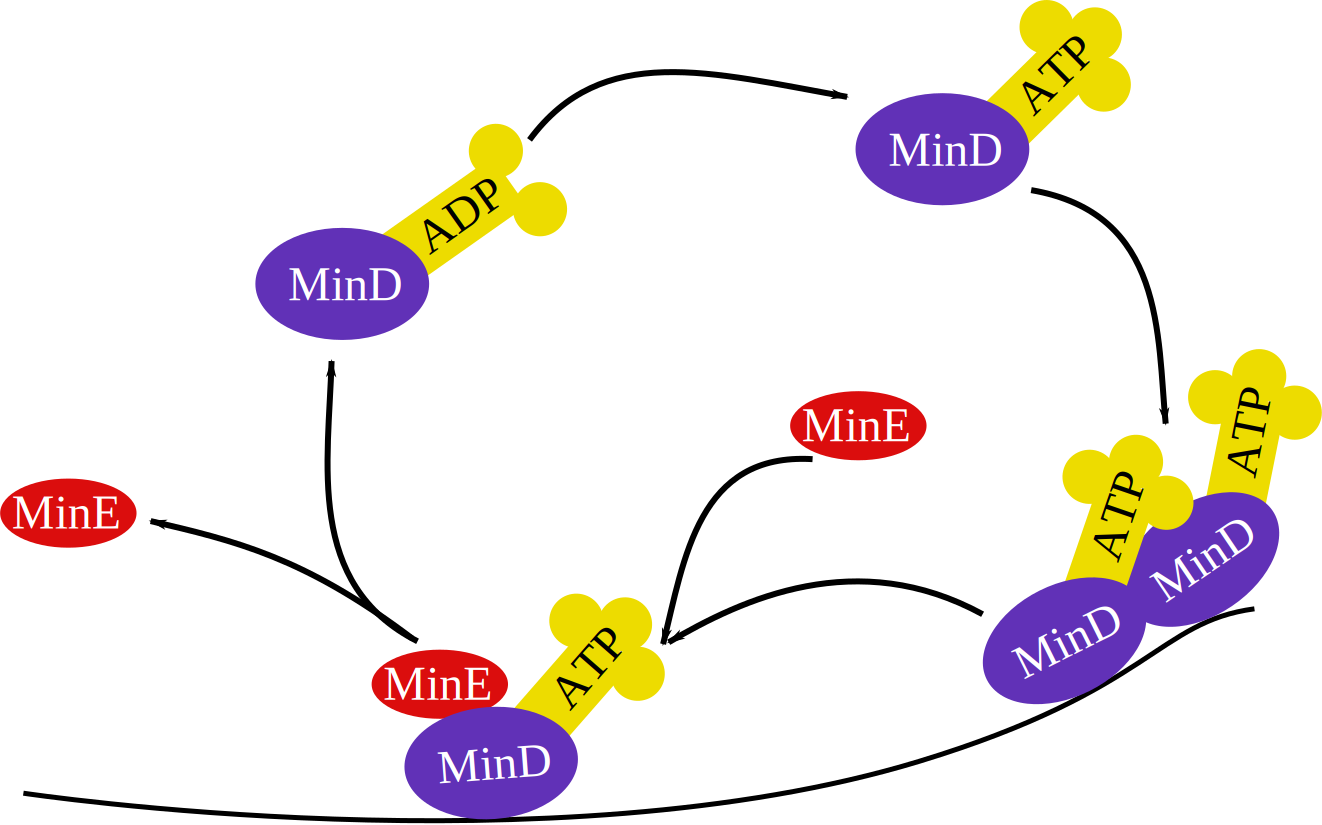
\includegraphics[width=8.7cm]{reactions}
  \caption{Reactions included in the Min system model of Huang
    \emph{et al.}, which is used in this
    work~\cite{huang2003dynamic}.}\label{fig:reactions}
\end{figure}


% You may title this section "Methods" or "Models". 
% "Models" is not a valid title for PLoS ONE authors. However, PLoS ONE
% authors may use "Analysis" 
\section*{Materials and Methods}
\subsection*{Model and Cell Shapes}
\label{sec:model-method-shapes}
We implement the reaction-diffusion model of Huang \emph{et
  al.}~\cite{huang2003dynamic}.  Figure~\ref{fig:reactions} shows the
reaction process.  The cytoplasmic MinD:ADP complex undergoes
nucleotide exchange and is changed into the MinD:ATP complex.  This
will naturally diffuse and attach to the cell membrane.  A cytoplasmic
MinE will attach to the wall bound MinD:ATP complex and after a time
will activate ATP hydrolysis.  This breaks up the complex, releasing
MinE, phosphate, and MinD:ADP back into the cytoplasm.  The MinD:ADP
will undergo nucleotide exchange and begin again the cyclic process.
The model is defined by a set of five reaction-diffusion equations:

\begin{align}
  \frac{\partial \rho_{D:ADP}}{\partial t} = \mathcal{D}_D\nabla^2\rho_{D:ADP}-k_D^{ADP\rightarrow ATP}\rho_{D:ADP}+\delta(d_w)k_{de}\sigma_{DE},\hspace{3.4cm}
\end{align}
\begin{align}
  \frac{\partial \rho_{D:ATP}}{\partial t} = \mathcal{D}_D\nabla^2\rho_{D:ATP}+k_D^{ADP\rightarrow ATP}\rho_{D:ADP}-\delta(d_w)[k_D+k_{dD}(\sigma_D+\sigma_{DE})]\rho_{D:ATP}
\end{align}
\begin{align}
  \frac{\partial \rho_E}{\partial t} = \mathcal{D}_E\nabla^2\rho_E+\delta(d_w)k_{de}\sigma_{DE}
  -\delta(d_w)k_E \sigma_D \rho_E
\end{align}
\begin{align}
  \frac{\partial \sigma_D}{\partial t} &= -k_E\sigma_D\rho_E
  +[k_D+k_{dD}(\sigma_D+\sigma_{DE})]\rho_{D:ATP}
  \label{eq:d-on-wall}
\end{align}
\begin{align}
  \frac{\partial \sigma_{DE}}{\partial t} &= -k_{de}\sigma_{DE}+k_E\sigma_D\rho_E\hspace{3cm}
  \label{eq:FifthPDE}
\end{align}
where $\rho$ is cytoplasmic protein density (proteins$/\micron^{3}$), $\sigma$
is membrane bound density (proteins$/\micron^{2}$), $\mathcal{D}_D$ and
$\mathcal{D}_{E}$ are the diffusion constants for MinD and MinE,
respectively, $k_D^{\textrm{ADP $\rightarrow$ ATP}}$ is the rate of
conversion from MinD:ADP to the MinD:ATP complex, $k_D$ is the rate of
MinD:ATP attachment to the membrane when no protein is already
attached there, $k_{dD}$ is the increase of this rate when MinD:ATP is
present on the membrane, $k_{de}$ is the rate of hydrolysis of the
MinD:MinE:ATP complex, $k_E$ is the rate of cytoplasmic MinE binding
to membrane bound MinD:ATP complex, and $d_w$ is the distance from the
point in space to the closest wall.  The Dirac delta function
$\delta(d_w)$, which we need to describe the location of the membrane,
has units of $\micron^{-1}$ and is zero everywhere except at the wall.
Equations \ref{eq:d-on-wall} and \ref{eq:FifthPDE} are only relevant
at the membrane because the membrane-bound density values have no
meaning in the cytoplasm.

Our diffusion and reaction rates are shown below.  We are interested
primarily in the effect of cellular size and shape on the protein
oscillations, so we use Huang's parameter
values~\cite{huang2003dynamic}.

\begin{gather*}
  \mathcal{D}_D = \mathcal{D}_{E} = 2.5\micron^2/\text{sec}\\
  k_D^{\textrm{ADP $\rightarrow$ ATP}} = 1/\textrm{sec,  }
  k_D = 0.025 \micron /\textrm{sec}\\
  k_{dD} = 0.0015 \micron^3/ \textrm{sec,  }
  k_{de} = 0.7/\textrm{sec}\\
  k_E = 0.093 \micron^3 /\textrm{sec}.
\end{gather*}

Huang's simulations use total MinD and MinE concentrations of
$1,000/\micron$ and $350/\micron$, respectively, in a cylindrical cell
of radius $0.5\micron$, and in our (non-cylindrical) cells we use the
same number of proteins per unit volume.  These concentration values
are $1273\micron^{-3}$ and $446\micron^{-3}$, respectively. We have
written our own simulation platform and membrane creation tools from
scratch, instead of using existing available software used in previous
studies~\cite{bonny2013membrane,fange2006noise,halatek2012highly,kerr2006division}.
Our simulations take place within a three-dimensional Cartesian grid
that has a grid spacing of .05\micron, and our cell shapes are
specified as the zero of an analytic function which can generate the
geometry presented in this paper.  This code is publicly available
on github~\cite{git}, including scripts that generate the simulation
data used in this paper.

We have performed both a numerical, deterministic model simulation
that is spatially and temporally discrete, and a stochastic simulation
that is spatially discrete but continuous in time.  Our stochastic
model follows the work of Kraus~\cite{kraus1996crosstalk} which in
turn follows a method introduced by
Gillespie~\cite{gillespie1977exact}.

We mean to investigate the geometric limits of the Min system
oscillations as observed by M\"annik \emph{et
  al.}~\cite{mannik2012robustness}, so we have modeled the Min system
in several cell shapes and sizes.  Here we present a selection of
these, beginning with naturally occurring pill-shaped cells, followed
by a number of flattened out shapes which reflect the experiments of
M\"annik \emph{et al.}, in which bacteria are confined within thin
slits.  These slits are fabricated with a width of .25\micron, but
they are coated with a PDMS lining that the cells are able to deform,
raising uncertainty in the actual cell thickness.  Tests with pure
silicon, non-deformable slits show that the smallest thickness for
which cells are able to penetrate is
.4\micron~\cite{mannik2012robustness,mannik2009bacterial}.  We
therefore assume that the PDMS slits have been deformed to this
thickness and simulate flattened cells with a thickness of .4\micron.
Viewed from the top down the cells have the shapes described below and
viewed from the side they have at their edges a semicircular
cross-section (one may imagine the shape of a pancake).
%
In this paper we focus on four specific flattened cell shapes.  Two of
these shapes replicate those published by M\"annik \emph{et al.}, and
the other two are `stadium' shapes that respectively have the same
aspect ratio, thickness, and volume as the two cell shapes
experimentally observed by M\"annik \emph{et
  al.}~\cite{mannik2012robustness}.  Viewed from the top down, these
stadium shapes appear as rectangles with semi-circular end caps on the
long axis ends.

\begin{figure*}
  %\includegraphics[width=\textwidth]{../data/shape-p/3_00-0_50-0_00-0_00-15_00-exact/plots/image-plot}
  \begin{center}
    \hspace{-3.5cm}
    \includegraphics[height=6.4cm]{../data/shape-p/3_00-0_50-0_00-0_00-15_00-exact/plots/single-image-plot}\\
    \vspace{-1.5em}
    \hspace{-3.5cm}
    \includegraphics[height=6.4cm]{../data/shape-p/3_00-0_50-0_00-0_00-15_00-full_array/plots/single-image-plot}
    \vspace{-1.5em}
  \end{center}
  \caption{Images of the concentration of each protein species in a
    natural pill-shaped bacterium at one-second time intervals. The
    upper plots shows results from the deterministic model and the
    lower shows results from the stochastic model.  The order of
    frames is such that individual MinD proteins begin at the bottom
    of the plot (in the MinD:ATP state in the cytoplasm), and progress
    upward until they reach the MinE:MinD:ATP membrane-bound complex.
    At that point, they will spontaneously dissociate into cytoplasmic
    MinE (the top row) and the starting state of cytoplasmic
    MinD:ADP.}.
  \label{image-p}
\end{figure*}


Huang \emph{et al.}~\cite{huang2003dynamic} have performed a linear
stability analysis on a cylindrical model which shows an upper limit
on a steady state solution of a $2\micron$ half wavelength.  Cells
with dimensions longer than this spontaneously develop spatial
oscillations, while cells that are shorter relax into a homogeneous
steady state.  We have performed a similar linear stability analysis
on an infinite slab with a thickness equal to that of our flattened
cells ($0.40\micron$).  We first solve the model's five differential
equations for the steady state solution, under the constraint that the
total number MinD and MinE molecules matches our simulation.  We write
down as a matrix the linear response of the time derivatives of the
density to small, spatially harmonic density perturbations around the
steady-state density.  The system is stable at this wavelength
provided all eigenvalues of the matrix are negative, indicating that
all perturbations with this wavelength will decay.  We find the
stability limit by searching for the largest wavelength at which the
system is stable.  Through this method we arrive at an upper half
wavelength stability limit of $1.56\micron$ for our $0.40\micron$
flattened cells. As expected, when decreasing the lengths and widths
of our simulated flattened cells so that the longest distance across
the cell is less than this length, the cells stop exhibiting any
oscillatory behavior.  The deterministic model relaxes into a
motionless state and the stochastic model exhibits random fluctuations
without spatial oscillations.

% Results and Discussion can be combined.
\section*{Results and Discussion}
\subsection*{Naturally Occurring Pill Shaped Cells}


\begin{figure}
  \begin{center}
    \includegraphics[height=6.4cm]{../data/shape-p/3_00-0_50-0_00-0_00-15_00-full_array/plots/correlation.pdf}
  \end{center}
  \caption{Temporal correlation function of the total MinD found in
    two opposite polar regions of the pill-shaped cell, shown against
    the correlation time.  Data for both the the deterministic and
    stochastic models are shown.  The stochastic model shows an
    oscillation period of 39.5 seconds and coherence time of 307 seconds.
    The correlation functions are scaled to have the same initial
    value.}
  \label{corr-pill}
\end{figure}

We begin with the naturally occurring pill cell shape.  We piece this
shape together as a cylinder with hemispherical end caps.  This shape
follows the early simulations of Huang \emph{et al.} but differs in
that we have added the end caps for a more natural shape, expecting
similar results.

Figure~\ref{image-p} shows a series of color plots of the density of
proteins at each stage of the reaction cycle. Deterministic simulation
data is shown above and stochastic simulation data is shown below.
The cells shown are $4\micron$ in length, measured from end to end.
We have `smeared out' the stochastic concentrations in a manner meant
to reproduce the images shown by diffraction limited fluorescence
microscopy.  We do so using the two dimensional Gaussian approximation
developed by Zhang \emph{et al.}~\cite{zhang2007gaussian}.  In this
approximation we use a numerical aperture value of 1.3, which is the
same as used by M\"annik experimentally, and a wavelength of $650nm$.
Each frame is 2.5 seconds ahead of the last, and each image shows the
concentration of a given state of protein (of the five described in
the reaction model) summed over the coordinate normal to the page.

Figure~\ref{image-p} begins about 300 seconds into the simulation and
shows one period of oscillation.  At $t=0$ there is a high
concentration of MinD:ATP that has accumulated on the membrane at the
bottom of the cell. An important aspect of Huang's model is that the
MinD is attracted to and sticks to the membrane nonlinearly: as it
accumulates there it begins to `recruit' other MinD that is diffusing
in the cytoplasm nearby, causing peaks in concentration to build up on
the walls.  Meanwhile, the MinE creeps downward as it reacts with the
membrane-bound MinD, forming the MinD:MinE:ATP complex, then breaks it
apart and diffuses downward a bit more before it again reacts with
membrane-bound MinD.  This process can be seen in the form of the
well-known ``MinE rings'' (actually, MinE bound to MinD on the
membrane).  These rings are visible in the deterministic model plots
as a green band on the walls from 0 seconds to 4 seconds (and later
from 15 to 23 seconds).  The appearance of these rings in the
deterministic model alongside their less obvious appearance in the
stochastic model highlights an advantage of the deterministic model:
the idealization of deterministic data allows one to see patterns in
the averaged behavior that might otherwise be missed.  In the
stochastic model the MinE still exhibits higher concentrations in the
same regions throughout the process, but what would ideally be a
``ring'' pattern is instead an asymmetric collection of maxima, which
would become a ring after phase-locked averaging.

During the formation of these rings, cytoplasmic MinE is diffusing in
the upper portion of the cell and will naturally progress downward,
where there is membrane-bound MinD to react with, leading to a
depletion of MinE in the upper portion of the cell.  As the MinE ring
converges upon the lower end of the cell, MinD that has been released
is able to diffuse upward, past the ring, while still in its MinD:ADP
state and unable to bind to the membrane.  After it undergoes
nucleotide exchange, resulting in MinD:ATP, it is ready to accumulate
on the walls in at the top of the cell, where the MinE has been
depleted.  This can be seen in seconds 10 through 20 in both models,
followed by the subsequent MinE ring formation and movement upward
(beginning the same process in the opposite direction) that can be
seen in seconds 15 through 23.

Both Fig.~\ref{image-p} and its associated movies (see supplementary
material), show that the stochastic model exhibits a ``starry night''
effect characterized by spatially fixed points of protein density
build up, as recruitment leads to clusters of MinD forming on the wall
and then subsequently dissipating.  This results from the omission of
diffusion along the membrane from Huang's model, which would allow
these recruitment clusters to spread out.  Experiments have confirmed
that diffusion along the membrane does occur, albeit with a rate two
orders of magnitude lower than that in the
cytoplasm~\cite{meacci2006mobility}.  The `stars' in the effect typically
last for around 10 seconds. The membrane-bound proteins will diffuse
by a distance of around one micron during this time, which is enough
to spread out across the polar section of the one micron diameter
wild-type pill cells.  As we see below, the flattened, irregular cells
are large enough that this one micron blurring would not completely
eliminate this `starry night' effect.

%% \fixme{calculating
  %% with $<x^2> = Dt$ and $D_{membrane} = .16\mu^2/s m$, which is just
  %% the experimental cytoplasmic value divided by 100, yields 1.2
  %% microns, which maybe is too high for what we're trying to say?
  %% Halatek uses $D_{membrane} = .013\mu^2/s m$, for which the same
  %% calculation would give .36 microns, which is better.  Halatek
  %% doesn't say why he uses a value that seems to be different than what
  %% Meacci claim to have found.  Halatek just says it's experimentally
  %% valid and cites their work.  What to do?}

We also analyze the temporal periodicity of the system, which we
quantify with the temporal correlation function of the total MinD
found in two opposite polar regions.  This correlation function, which
is displayed in Fig.~\ref{corr-pill}, is given by
\begin{equation}
  C(\tau) \propto \int
  (N_{\textit{top}}(t) - \bar N_{\textit{top}})
  (N_{\textit{bottom}}(t+\tau) - \bar N_{\textit{bottom}})dt
\end{equation}
where $N_{\textit{top}}(t)$ and $N_{\textit{bottom}}(t)$ are the total
MinD proteins in the top and bottom thirds of a cell.  These plots
help us in studying the periods and the regularity and stability of
oscillations.  These curves are well fit with a simple decoherence
model, given by the equation
\begin{equation}
  C(\tau) = -\cos\left(\frac{2\pi\tau}{T}\right) e^{-\frac{\tau}{\tau_c}}
\end{equation}
where $T$ is the period and $\tau_c$ is the coherence time.  In the
case of the stochastic model the pill exhibits coherence times of
about 8 periods, indicating that the system exhibits periodic
oscillation, with some stochastic irregularity in the period.
%
In contrast, in the deterministic model the pill-shaped cell exhibits
complete coherence, indicating that its behavior is perfectly
periodic.

\begin{figure*}
  \centering
  \hspace{-3cm}
  \vspace{1cm}
  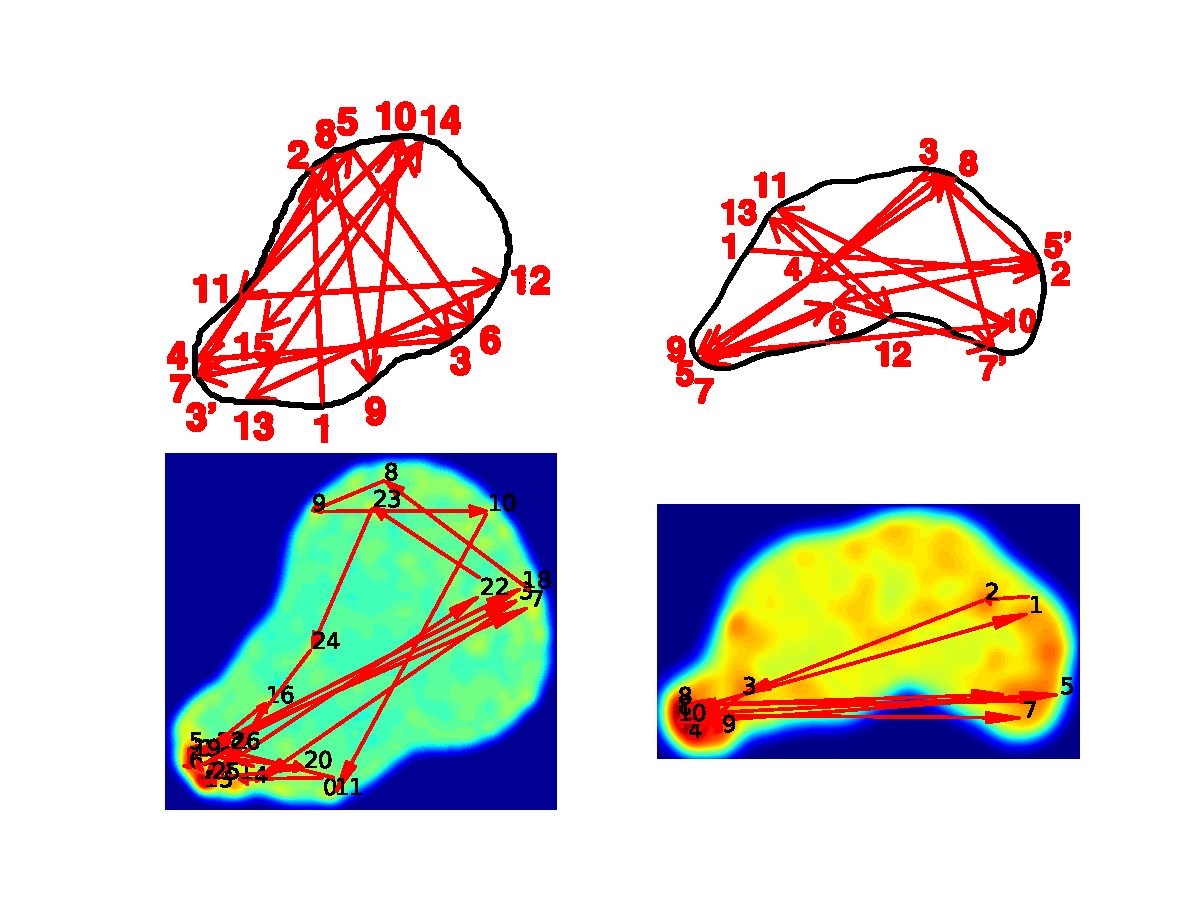
\includegraphics[width=16cm]{../paper/plot-ave}
  \caption{Arrows depicting successive maxima in space
    and time overlayed on a color plot of the total MinD density
    averaged over the same time period.  The simulation time covered
    for the flattened cells is 350 seconds, which is the same
    period of time depicted in the experimental data plots of M\"annik
    \emph{et al.}~\cite{mannik2012robustness}.  For the wild-type pill
    shape, we only cover 250 seconds, in order to provide a
    useful comparison due to its shorter oscillation period.  The top
    row shows plots published by M\"annik \emph{et al.} of the MinD maxima behavior
    and the bottom two rows show our simulations using the stochastic
    and deterministic models, respectively.  We simulated
    approximations to the two shapes observed by M\"annik, which we call
    \emph{shape A} and \emph{shape B}.  In addition, we studied two
    flattened stadium shapes which we call \emph{stadium A} and
    \emph{stadium B} corresponding in aspect ratio and thickness to
    the two experimental shapes.  The spatial length scale of all the
    figures shown was identical. Each of the flattened cell shapes
    uses the same color scale for the number of proteins per unit
    area.  Finally, we display the natural pill shape, which was also
    featured in Figs.~\ref{image-p} and~\ref{corr-pill}, with a
    different color scale to reflect the thicker cell containing more
    proteins per cross-sectional area.  }
  \label{randst-plot-ave}
\end{figure*}

%% \begin{figure}
%%   \begin{center}
%%     \includegraphics[height=6.4cm]{../data/shape-randst/0_40-18_50-18_50-95_00-15_00-full_array/plots/correlation.pdf}\\
%%     \includegraphics[height=6.4cm]{../data/shape-stad/0_40-2_35-1_32-0_00-15_00-full_array/plots/correlation.pdf}
%%   \end{center}
%%   \caption{Temporal correlation function of the total MinD found in
%%     two opposite polar regions of the shape \emph{A} (above) and the
%%     stadium \emph{A} (below) cell shapes, shown against the
%%     correlation time.  Data for both the the determinisitic and
%%     stochastic models are shown, and the correlation functions are
%%     scaled to have the same initial value.  For shape \emph{A}, the
%%     stochastic model shows an oscillation period of 52 seconds and
%%     coherence time of 288 seconds, so that it takes roughly 5.5
%%     periods for the behavior to decohere.  For the stadium \emph{A},
%%     the same model shows an oscillation period of 48.4 seconds and
%%     coherence time of 638 seconds, so that it takes roughly 13
%%     periods for the behavior to decohere.}
%%   \label{fig:corr-pancake-A}
%% \end{figure}


\begin{figure}
  \begin{center}
    \includegraphics[width=8.7cm]{../data/shape-randst/0_40-18_60-28_60-94_00-15_00-full_array/plots/correlation.pdf}
    \includegraphics[width=8.7cm]{../data/shape-stad/0_40-2_92-1_18-0_00-15_00-full_array/plots/correlation.pdf}
  \end{center}
  \caption{Temporal correlation function of the total MinD found in
    two opposite polar regions of the shape \emph{B} (above) and the
    stadium \emph{B} (below) cell shapes, shown against the
    correlation time.  Data for both the the deterministic and
    stochastic models are shown, and the correlation functions are
    scaled to have the same initial value.  For shape \emph{B}, the
    stochastic model shows an oscillation period of 58 seconds and
    coherence time of 306 seconds, so that it takes roughly 5.3 periods
    for the behavior to decohere.  For the stadium \emph{B}, the same
    model shows an oscillation period of 51 seconds and coherence time
    of 442 seconds, so that it takes roughly 8.6 periods for the
    behavior to decohere.}
  \label{fig:corr-B}
\end{figure}



\subsection*{Comparison of Experimental and Stadium Shapes}
%\label{sec:model-method-shapes}
As explained above, we focus on simulation of four illustrative
flattened cell shapes: two shapes created to replicate those shapes
observed experimentally by M\"annik \emph{et
  al.}~\cite{mannik2012robustness} (shape~\emph{A} and
shape~\emph{B}), and for comparison two `stadium' shapes that have the
identical aspect ratio, thickness and volume (stadium \emph{A} and
stadium \emph{B}), shown in Figure~\ref{randst-plot-ave}.  All of the
flattened cells have lost the rotational symmetry of the original pill
shapes, but while shape~\emph{A} and shape~\emph{B} have only one
mirror plane symmetry (that is normal to the flattened plane),
stadium~\emph{A} and stadium~\emph{B} have three.  This allows us to
distinguish between the effect of flattening the cell and the cell
shape's irregularity and asymmetry.

%% For each of these shapes (in
%% addition to the wild-type pill shape discussed previously) we have
%% simulated in excess of 15000 seconds (over 4 hours) of evolution of
%% the MinD system using the deterministic version of Huang's
%% model~\cite{huang2003dynamic}, and in excess of 100000 seconds (over
%% 27 hours) using the stochastic model.

From each of these flattened simulations, we have chosen a typical 350
second segment to compare with the published results of
M\"annik \emph{et al.}~\cite{mannik2012robustness}, exemplified in arrow plots in
which the arrow heads show the location of sequential MinD maxima
within the cell (in Fig.~\ref{randst-plot-ave}).  In addition to
arrows between successive maxima in space and time, we plot as a
colored background the density of MinD proteins averaged over the same
time period.  We note that we have manually verified that our
(computer-generated) arrow plots also reflect a human interpretation
of a movie of the same data.  Finally, for comparison we present the
same plot for a wild-type cell, with a time period of 250 seconds to
account for its short period of oscillation.

In every case, including the wild-type pill shape, we see irregularity
in the location of the maxima when using the stochastic model.  The
deterministic model shows uniformly bipolar oscillation.  We conclude
that this model is \emph{not} chaotic (which would show irregularity
in the deterministic computation), but rather that the irregularity
results purely from stochastic processes.  From these results and how
they compare with experiment, we conclude that the deterministic model
is inadequate to explain experimental observations of the locations of
density maxima of the MinD protein.  We note, however, that it is
possible that there exists another deterministic model that does exhibit
chaotic behavior.

%% We found that the deterministic simulations of the MinD system results
%% in robust and regular oscillatory behavoir of polar selection and
%% oscillation in not only symmetrical shapes, such as the wildtype pill
%% shape, but also in very assymetrical, flatttened cells, such as those
%% observed by M\"annik.  We also examined larger and smaller versions of
%% these shapes, and found this behavior to be very robust, from the
%% minimum size to sustain oscillation (around \fixme{???} $\mu$m) up to
%% around twice the cell size reported by M\"annik.  At larger sizes than
%% this, less regular oscillations occur using the deterministic method,
%% but we note that the cells reported by M\"annik are already considerably
%% larger in volume than typical wild type
%% cells~\cite{kubitschek1990cell,kubitschek1968linear,mannik2012robustness}.

The predictions of the stochastic model show some similarity to the
experimental results in terms of irregularity of the locations of
maxima, but the stochastic model displays significantly less
variation in the direction of oscillations than experiment, suggesting
inadequacies in the model.  We also note that the stadium shapes in
Fig.~\ref{randst-plot-ave} appear to have maxima location irregularity
that is qualitatively similar to our irregular shapes: in both
stochastic simulations the overall oscillation is largely bipolar, but
with irregularity in the locations of the maxima that form at each
end.

However Fig.~\ref{randst-plot-ave} leaves unclear the importance of
the flattening and accompanying lateral expansion of the cell versus
cell shape irregularity and asymmetry in the temporal regularity of
the oscillations.  Although in the movies the stadiums appear to
display, on average over long time scales, a somewhat more regular
oscillation than appears in the irregular shapes \emph{A} and
\emph{B}, the limited time range of the arrow plots (350 seconds) is
inadequate to make this comparison.  We therefore return to the
correlation function between the number of proteins in a segment at
the top of the cell and the number of proteins in a segment at the
bottom of the cell.  Fig.~\ref{fig:corr-B} shows this plot for shape
\emph{B} and stadium \emph{B}.  Here we plot correlations of
correlation times up to 500 seconds, a biologically relevant
timescale.  E. Coli cell doubling times vary widely depending on
environmental conditions, but will often be between 20 minutes to 100
minutes~\cite{pierucci1972chromosome}, while fluorescent microscopy
experiments have shown that the FtsZ ring builds itself with a half
life of roughly 30 seconds~\cite{stricker2002rapid}.

We see that both in the shape \emph{B} and stadium \emph{B}, the
deterministic model is perfectly periodic.  Both the deterministic and
stochastic model correlations have the same number of proteins in
their cells, and have been normalized with the same normalization
factor, so that they can be directly compared against each other.  The
stochastic simulation of shape \emph{B} has a coherence time of 5.3
periods, while the corresponding simulation of stadium \emph{B} has a
coherence time of 8.6 periods.
%
The correlation function for stadium \emph{A} is similar to that of
stadium~\emph{B}, with similar coherence time (13 periods, not shown),
while shape~\emph{A} also exhibits a similar coherence time (5.5
periods).  This confirms that the stadium shapes do indeed oscillate
somewhat more regularly than the irregular shapes, but both are
comparable to the wild-type pill shape.
%
From the stochastic correlation data, we conclude that irregularity of
shape leads to a decrease in temporal regularity of the oscillatory
behavior, although even the very distorted shape~\emph{B} exhibiting
only a factor of two greater decoherence.

\section*{Conclusion}
We find agreement between our stochastic simulations and experiments
showing disrupted bipolar MinD oscillation in asymmetric flattened
E. coli cells~\cite{mannik2012robustness}.  As observed
experimentally, our simulations predict that MinD maxima will form in
a spatially irregular sequence of locations.  This result builds upon
existing results showing that this model and its variants are
effective in a variety of wild-type and mutated cell
shapes~\cite{fange2006noise, varma2008min, kruse2007experimentalist},
and reinforces that stochastic variations of Huang's 2003
model~\cite{fange2006noise, kerr2006division} has considerable
predictive power beyond the standard wild-type cell.

In contrast to the stochastic model, the original deterministic
version of the model~\cite{huang2003dynamic} predicts behavior that
contradicts experimental observations.  Specifically, the
deterministic model predicts robust and periodic bipolar oscillation
in irregularly shaped cells.  Thus we conclude that this method is
inconsistent with experiment, and cannot be relied upon for
predictions of the behavior of the MinD system.  This is the most
clear example of the inadequacy of the deterministic simulation method
in reproducing experimental behavior of the MinD system to date.
Until now the results of deterministic and stochastic simulation have
largely coincided, with the stochastic method showing minor
differences in behavior when compared to deterministic
models~\cite{kerr2006division, fange2006noise, huang2004min,
  kruse2007experimentalist}.  The regular oscillations in the
deterministic case also allow us to conclude that Huang's model is
non-chaotic.  Because of their similar construction, we anticipate
that recent variants of the model~\cite{bonny2013membrane,
  fange2006noise, halatek2012highly} may also prove to be
non-chaotic.

We find that flattened but regular and symmetric cells exhibit MinD
oscillations that are qualitatively similar to the oscillations
observed experimentally (and in our simulation) in irregular and
asymmetric cells.  This demonstrates that asymmetry is not required in
order to induce spatially irregular MinD oscillations.  In addition,
the temporal regularity of oscillations is only moderately affected by
irregularity in the shape of flattened cells.  Thus we conclude that
it may be the flattening of the cells, and the accompanying
expansion in the transverse direction, that causes the disruption of
regular bipolar oscillation which is observed by M\"annik \emph{et
  al.}~\cite{mannik2012robustness}.


\section*{Supporting Information}

% Include only the SI item label in the subsection heading. Use the \nameref{label} command to cite SI items in the text.
\subsection*{S1 Video}
\label{movie-MinD-density-pill}
{\bf Movie that shows the evolution of MinD density over a 250 second
  interval in a wild-type, pill-shaped cell.}  There is one frame for
every half second of simulation time. Above are results from the
stochastic model and below are results from the deterministic model.
The density shown is integrated over the direction normal to the
screen, so that the data is shown in molecules/$\micron^2$.

\subsection*{S2 Video}
\label{movie-MinD-density-shape-A}
{\bf Movie that shows the evolution of MinD density over a 350 second
  interval in the shape A cell.}  There is one frame for every half
second of simulation time. Above are results from the stochastic model
and below are results from the deterministic model.  The density shown
is integrated over the direction normal to the screen, so that the
data is shown in molecules/$\micron^2$.

\subsection*{S3 Video}
\label{movie-MinD-density-shape-B}
{\bf Movie that shows the evolution of MinD density over a 350 second
  interval in the shape B cell.}  There is one frame for every half
second of simulation time. Above are results from the stochastic model
and below are results from the deterministic model.  The density shown
is integrated over the direction normal to the screen, so that the
data is shown in molecules/$\micron^2$.

\subsection*{S4 Video}
\label{movie-MinD-density-stadium-A}
{\bf Movie that shows the evolution of MinD density over a 350 second
  interval in the stadium A cell.}  There is one frame for every half
second of simulation time. Above are results from the stochastic model
and below are results from the deterministic model.  The density shown
is integrated over the direction normal to the screen, so that the
data is shown in molecules/$\micron^2$.

\subsection*{S5 Video}
\label{movie-MinD-density-stadium-B}
{\bf Movie that shows the evolution of MinD density over a 350 second
  interval in the stadium B cell.}  There is one frame for every half
second of simulation time. Above are results from the stochastic model
and below are results from the deterministic model.  The density shown
is integrated over the direction normal to the screen, so that the
data is shown in molecules/$\micron^2$.

% Do NOT remove this, even if you are not including acknowledgments.
\section*{Acknowledgments}

\nolinenumbers

% Compile your BiBTeX database using our plos2009.bst
% style file and paste the contents of your .bbl file
% here.

\bibliography{paper-MinD}


\end{document}

